\def\datum{Version of 20.07.2015} 
% 
% 
\documentclass[smallextended]{svjour3} 

\usepackage{tikz}		% for graph drawing 
\usepackage{subfigure}	% for subfigures 
\usepackage{placeins}	% float barrier 

\usepackage{graphicx} 
\usepackage{amsmath} 
\usepackage{amssymb} 
\usepackage{a4wide} 
\usepackage{comment} 

% 
% please place your own definitions here and don't use \def but 
% \newcommand{}{} 
\newtheorem{algorithm}{Algorithm} 
% 
% Definitions 
\def\dist{\mathop{\rm dist}} 
\def\deg{\mathop{\rm deg}} 

% ToDo 
\usepackage{xcolor} 
\newcommand\ToDo[1]{\textcolor{red}{#1}} 
% 
% Insert the name of "your journal" with 
\journalname{Journal} 
% 
\begin{document} 
\title{Computation of Optimum Distance Constrained Labelings} 
\author{Veronika Hal\'asz \and Gerhard Reinelt \and Ekaterina Tikhoncheva} 
\authorrunning{V.~Hal\'asz, G.~Reinelt, E.~Tikhoncheva} 
\institute{Institut f\"ur Informatik, Universit\"at Heidelberg\\ 
Im Neuenheimer Feld 368, 69120 Heidelberg, Germany\\ 
%\email{} 
} 

\date{\datum} 

\maketitle 

\begin{abstract} 
There are many problems in graph theory concerned with labeling the 
vertices of a graph subject to certain constraints and opimization criteria. In this 
paper we study so-called distance constrained labeling problems where, depending on 
the distance between two vertices, lower bounds on the difference 
between their (integer or continuous) labels have to observed. We discuss integer programming 
approaches for finding labelings with minimum spans and report about computational 
experiments. 
\end{abstract} 

\keywords{Graphs \and Labeling} 

% 
% 
% 
\section{Introduction} 
 
Many problems in graph theory deal with the assignment of colors or labels to the vertices 
of a given graph satisfying certain constraints and optimizing some objective function. 
Prominent examples are \emph{coloring problems} like the determination of the minimum 
number of colors necessary such that two adjacent vertices have different colors 
or \emph{labeling problems} where labels correspond to integer numbers and where 
the difference between labels plays a role. 

A special type of labeling problems, so-called 
\emph{distance constrained labeling problems}, have been introduced by Hale~\cite{Hal80}. 
They are motivated by the problem of assigning frequencies to radio channels in order 
to avoid interference. In Hale's approach channels (frequencies) are 
represented by nonnegative integers and have to be assigned to transmitters. 
Close transmitters should receive different frequencies and very close 
transmitters should receive frequencies further apart. The bandwidth of an assignment 
is the maximum absolute difference between frequencies and should be as small 
as possible. 

The problem can be modeled as a graph labeling problem. The vertices of 
the graph correspond to transmitters and the vertex labels to frequencies. 
Depending on the definition of the distance between two vertices several 
models are possible. At first we consider the classical version where 
the distance between two vertices is the smallest number of edges in a path connecting them. 

Let $G=(V,E)$ denote the (undirected) graph with vertex set~$V$, $|V|=n$, and edge set~$E$. 
In the most intensively studied model in this context, nonnegative 
integer labels have to be assigned to the vertices of~$G$, 
such that the labels of adjacent vertices must differ by at least~2 and 
vertices having common neighbors must get distinct labels. 
This so-called \emph{$L(2,1)-$labeling problem} 
was first investigated by Griggs and Yeh~\cite{GY92}. The smallest 
possible value of the largest label in such a labeling 
is denoted by $\lambda_{2,1}(G)$ (for example: see Fig.~\ref{fig:1}). 

% Fig 1 
\begin{figure}[ht]
\centering

	\vbox{ 
		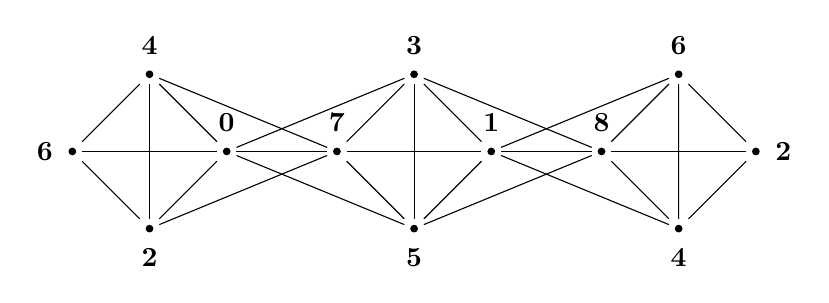
\begin{tikzpicture}[scale=0.7]

		\node[label=left: $\bf{ 6}$] (v1) at ( 0.0, 0.0) {};\fill (v1) circle (2pt);
		\node[label=above:$\bf{ 4}$] (v2) at ( 1.4, 1.4) {};\fill (v2) circle (2pt);
		\node[label=above:$\bf{ 0}$] (v3) at ( 2.8, 0.0) {};\fill (v3) circle (2pt);
		\node[label=below:$\bf{ 2}$] (v4) at ( 1.4,-1.4) {};\fill (v4) circle (2pt);
		
		\node[label=above:$\bf{ 7}$] (v5) at ( 4.8, 0.0) {};\fill (v5) circle (2pt);
		\node[label=above:$\bf{ 3}$] (v6) at ( 6.2, 1.4) {};\fill (v6) circle (2pt);
		\node[label=above:$\bf{ 1}$] (v7) at ( 7.6, 0.0) {};\fill (v7) circle (2pt);
		\node[label=below:$\bf{ 5}$] (v8) at ( 6.2,-1.4) {};\fill (v8) circle (2pt);
	
		\node[label=above:$\bf{ 8}$] (v9)  at ( 9.6, 0.0) {};\fill (v9) circle (2pt);
		\node[label=above:$\bf{ 6}$] (v10) at ( 11.0, 1.4) {};\fill (v10) circle (2pt);
		\node[label=right:$\bf{ 2}$] (v11) at (12.4, 0.0) {};\fill (v11) circle (2pt);
		\node[label=below:$\bf{ 4}$] (v12) at ( 11.0,-1.4) {};\fill (v12) circle (2pt);

		\draw[-] (v1) to (v2); \draw[-]  (v1) to (v3); \draw[-]  (v1) to (v4);
		\draw[-] (v2) to (v3); \draw[-]  (v2) to (v4);
		\draw[-] (v3) to (v4);
		
		\draw[-] (v2) to (v5);
		\draw[-] (v3) to (v5);		
		\draw[-] (v4) to (v5);
		
    	\draw[-] (v6) to (v3);
		\draw[-] (v5) to (v3);		
		\draw[-] (v8) to (v3);
				
		\draw[-] (v5) to (v6); \draw[-]  (v5) to (v7); \draw[-]  (v5) to (v8);
		\draw[-] (v6) to (v7); \draw[-]  (v6) to (v8);
		\draw[-] (v7) to (v8);

		\draw[-] (v6) to (v9);
		\draw[-] (v7) to (v9);		
		\draw[-] (v8) to (v9);
		
    	\draw[-] (v10) to (v7);
		\draw[-] (v9) to (v7);		
		\draw[-] (v12) to (v7);
		
		\draw[-] (v9) to (v10); \draw[-] (v9) to (v11); \draw[-] (v9) to (v12);
		\draw[-] (v10) to (v11); \draw[-]  (v10) to (v12);
		\draw[-] (v11) to (v12);
		
	\end{tikzpicture}
	}
\caption{Example of the $L(2,1)-$labeling problem with $\lambda_{2,1}(G) = 8$.}
\label{fig:1}
\end{figure} 

More generally, an $L(j_1,j_2)-$labeling of $G$ is an assignment of nonnegative 
integer labels to the vertices of $G$ in such a way that the labels 
of vertices at distance 2 apart differ at least by $j_2$ and labels of adjacent 
vertices differ by $j_1$ or more. 
A comprehensive survey of $L(j_{1},j_{2})-$labeling and bounds on 
the minimum $\lambda_{j_{1},j_{2}}(G)$ of the largest label, with 
nearly 200 references, was given by Calamoneri in ~\cite{3}. 

As regards vertices at larger distances apart, $L(3,2,1)-$labeling 
(first studied by Shao and Liu in ~\cite{4}) and more generally $L(j_{1},j_{2},j_{3})$--labeling (introduced by Shao in ~\cite{5} put three conditions, depending on the distances between vertices. Here the parameter $j_{i}$ describes that the difference between the labels of vertices at distance $i$ apart must be at least $j_{i}$. The properties of $L(3,2,1)$--labelings 
have been analyzed further in ~\cite{6}. 
% 


The problem can be extended in a natural way to longer distances. 
Let $j_1,j_2,\ldots,j_{s}$ be nonnegative integers such that $j_1\geq j_2\geq\ldots\geq j_{s}$. An \emph{$L(j_1,j_2,\ldots,j_{s})-$labeling} of~$G$ is an assignment $\varphi:\: V\rightarrow\{0,1,2,\ldots\}$ such that for every pair $u$ and $v$ of vertices the inequality $|\varphi(u)-\varphi(v)|\geq j_{i}$ holds if the distance between $u$ and $v$ in $G$ is equal to $i$, for some $i=1,2,\ldots,s$. Note that there are no constraints for~$u$ and~$v$ if their 
distance is greater than~$j_s$ and that with this definition an $L(j_1,j_2)-$labeling can be considered as $L(j_1,j_2,0,0,\ldots)-$labeling. 
 
The \emph{span} of an $L(j_1,j_2,\ldots ,j_{s})-$labeling 
$\varphi$ is the largest label assigned by $\varphi$ to the vertices. 

In analogy to $\lambda_{2,1}$ we define $\lambda_{j_1,j_2,\ldots ,j_{s}}=\min_{\varphi}\max_{v\in V}\varphi(v)$ as the smallest possible span taken over all $L(j_1,j_2,\ldots ,j_{s})-$labelings~$\varphi$. 
This general labeling is less studied but there are some interesting results for a special case, 
namely for the radio-labeling in ~\cite{CEHZ,L,LMZ,HT}. A brief summary of the basic results with the related references is given in subsection 7.4 of the survey [G].

This paper deals with the computation of optimum distance constrained labelings. 
In section~\ref{sec:IP} we discuss models for the classical problem as 
well as for variants closer to real frequency assignment problems. Section 3 describes the graphs on which the tests were carried out. We present our first computational experiments in section 4 and the improvements in section 5. In the end of the paper we may draw some conclusions about the results.




\subsection{Computational complexity} 

It was already known from \cite{GY92} that the decision version of the simplest labeling $L(2,1)$ (that is, the input consists of a graph $G$ and an integer $k$, and the question is whether $\lambda_{2,1}(G)\leq k$ holds) on unrestricted input graphs is NP-complete. 

Fiala, Golovach and Kratochvil~\cite{7} proved that the decision version of the $L(j_{1},j_{2})-$labeling problem is NP-complete on trees whenever $j_{1}$ is not a multiple of $j_{2}$. Otherwise it is reducible to $L(\frac{j_{1}}{j_{2}},1)$, which is solvable in polynomial time~\cite{8} using the modificated algorithm of Chang and Kuo \cite{9}. This algorithm works not only on trees but also on the slightly wider class of graphs which can be transformed to a tree by removing at most $p$ edges for some fixed $p$. 

The $L(2,1)-$labeling problem still remains NP-complete for planar graphs, bipartite graphs, split graphs and chordal graphs~\cite{10}, even for graphs of treewidth 2~\cite{11}. In the case of planar graphs, deciding about the existence of a $k-L(2,1)-$labeling is NP-hard for $k\geq4$, while it can be done in polynomial time for $k\leq3$~\cite{12}. 


\section{Models for computing distance constrained labelings} 
\label{sec:IP} 

We start with an integer programming model for the classical problem. 
Let the label of vertex~$v$ be represented by the integer 
variable~$c(v)$ and let $\dist(u,v)$ denote the distance between two vertices $u$ and $v$. 

The problem of finding an optimum $L(j_1,j_2,\ldots ,j_{s})-$labeling 
can be stated as follows. 
\begin{alignat}{2} 
\min L      &                            & \quad & \notag\\ 
L-c(v)       &\;\ge\;0                    & \quad &\forall\, v\in V\label{ip:1}\\ 
|c(v)-c(u)| &\;\geq\;j_{\dist(u,v)} & & \forall\, u,v\in V\text{ with }{\dist(u,v)}\le j_s \label{ip:2}\\ 
c(v)          &\;\geq\;0                  & &\forall\, v\in V \label{ip:3}\\ 
c(v)          &\;\text{ integer}       & & \forall\, v\in V.\label{ip:4} 
\end{alignat} 

Inequalities~(\ref{ip:1}) model the min-max objective function and so 
$\min\lambda_{j_1,j_2,\ldots ,j_{s}}(G)$ is computed. The distance 
constraints~(\ref{ip:2}) for vertex pairs $u$ and $v$ can be linearized 
in the standard way with additional binary variables $z_{uv}$ as follows.

\begin{alignat}{2} 
c(v)-c(u)+M\cdot z_{uv}     &\;\geq\;j_{\dist(u,v)} & \quad& \forall\, u,v\in V\text{ with }{\dist(u,v)}\le j_s\notag\\ 
c(u)-c(v)+M\cdot(1-z_{uv}) &\;\geq\;j_{\dist(u,v)} &   &\forall\, u,v\in V\text{ with }{\dist(u,v)}\le j_s\notag\\ 
z_{uv}                                &\;\in\;\{0,1\}              &  & \forall\, u,v\in V.\notag 
\end{alignat} 

The number~$M$ has to be chosen big enough. Obviously 
$M\geq j_1+\lambda_{j_1,j_2,\ldots ,j_{s}}(G)$ has to hold. If no good upper bound 
on $\lambda_{j_1,j_2,\ldots ,j_{s}}(G)$ is known, we just set $M=n\cdot j_1$. 

The distance labeling problem introduced so far is an interesting 
graphtheoretical problem. However, it does not model a practical frequency 
assignment problem properly because the discrete graph distances do not 
reflect the real distances between transmitters. Hence it can only serve 
as a coarse approximation. 

A possibility for making the model more practical would be to 
insert artificial vertices to increase the distance between vertices 
closer to reality. This way we preserve the discrete nature of the model, 
but the graph size is increased. 

One could also allow real values as labels (leaving the graph and the distance 
unchanged). Since proper integer solutions remain feasible, 
the minimum span is not bigger than in the classical model. 
Actually, this is the LP relaxation of the model above. 
 We even can prove that the span is the same in the cases of integer and real labels. 


\paragraph{Theorem} 
If the required differences $j_1,j_2,\ldots ,j_{s}$ are each integers, then the labeling number is an integer and there exists an optimal labeling with integer labels. 

\paragraph{Proof} 
Let an optimal labeling $\varphi$ be given. Take the floor of each labels. In this way we get the integer labeling $\varphi_{i}$. Obviously, the biggest one of the new labels is not greater than before. In the following we prove that the requirements are met for each vertex pairs also in $\varphi_{i}$. 

Let $u$ and $v$ be arbitrary vertices of $G$, where without loss of generality we may assume that $\varphi(u)\leq\varphi(v)$. Then $\varphi(v)-\varphi(u)\geq d_{dist(u,v)}$ since $\varphi$ is a proper labeling. 

By definition $\varphi_{i}(v)=\left\lfloor \varphi(v)\right\rfloor =\varphi(v)-frac(\varphi(v))$, where $frac(\varphi(v))$ defines the fractional part of $\varphi(v)$. Similar holds for $u$, as well. So, $\varphi_{i}(v)+frac(\varphi(v))-\varphi_{i}(u)-frac(\varphi(u))\geq d_{dist(u,v)}$, 
where $d_{dist(u,v)}\in\mathbb{N}$. It means that $\varphi_{i}(v)-\varphi_{i}(u)+(frac(\varphi(v))-frac(\varphi(u)))\geq d_{dist(u,v)}$ 
$\Rightarrow\varphi_{i}(v)-\varphi_{i}(u)\geq d_{dist(u,v)}-(frac(\varphi(v))-frac(\varphi(u)))$. 


The greatest possible value of $(frac(\varphi(v))-frac(\varphi(u)))$ is $(1-\varepsilon)-0=1-\varepsilon<1$, the smallest possible one is $\varepsilon-1>-1$. Since $\varphi_{i}(v)-\varphi_{i}(u)$ is an integer, it is at least as large as $\left\lceil  d_{dist(u,v)}-(frac(\varphi(v))-frac(\varphi(u)))\right\rceil$. $d_{dist(u,v)}\in\mathbb{N}$ and $-1<(frac(\varphi(v))-frac(\varphi(u)))<1$. 

Hence $\left\lceil d_{dist(u,v)}-(frac(\varphi(v))-frac(\varphi(u)))\right\rceil =d_{dist(u,v)}$ 
$\Rightarrow\varphi_{i}(v)-\varphi_{i}(u)\geq d_{dist(u,v)}$. The same argument holds for each vertex pair, so $\varphi_{i}$ is a proper labeling with span not bigger than that of $\varphi$. Because of the optimality of $\varphi$, $\varphi_{i}$ is an optimal labeling using only integers. 

Some results about labeling with real numbers can be found in ~\cite{13}. 
It would be most precise to consider the complete graph on transmitters (nodes embadded in the 
plane) and to take the Euclidean distance between nodes 
as edge weights. Since the graph is finite there is also only a finite 
number, say~$t$, of occurring distances, and constraints could be formulated as above 
relative to a sequence $L(j_{dist_{1}},j_{dist_{2}},\ldots ,j_{dist_{t}})$. 

For the \emph{Euclidean model} we can basically adopt the integer model 
with two little changes. First, the variables $c(v)$ are now continuous. 
Second, the Euclidean distances have to be transformed to suitable right hand 
side values for the inequalities~(\ref{ip:2}). This will be accomplished by a 
function~$\ell(\dist(u,v))$. The principle formulation of the Euclidean approach is the following. 

\begin{alignat}{2} 
\min L      &                            & \quad & \notag\\ 
L-c(v)       &\;\ge\;0                    & \quad &\forall\, v\in V\notag\\ 
c(v)-c(u)+M\cdot z_{uv}     &\;\geq\;\ell(\dist(u,v)) & \quad& \forall\, u,v\in V\text{ with }{\dist(u,v)}\le j_s\notag\\ 
c(u)-c(v)+M\cdot(1-z_{uv}) &\;\geq\;\ell(\dist(u,v)) &   &\forall\, u,v\in V\text{ with }{\dist(u,v)}\le j_s\notag\\ 
c(v)          &\;\geq\;0                  & &\forall\, v\in V \notag\\ 
z_{uv}                                &\;\in\;\{0,1\}              &  & \forall\, u,v\in V.\notag 
\end{alignat} 

\section{Test instances} 

We are not aware of any research on solving distance constrained labeling problems 
to optimality with Euclidean distances between transmitters, so we generated own benchmark problems. The goal was to test the 
graph model and the Euclidean model on instances which somehow resemble the practical 
situation for real frequency assigment problems. 

In radio and mobile networks large areas are usually covered by polygons 
which together form lattices. In practice three lattices play a prominent 
role: square, hexagonal and triangular lattices (see Fig.\ref{fig:2}). 

% Fig 2 
\begin{figure}[hb]
\begin{minipage}[h]{0.33\linewidth}
	\centering
    \vbox{ 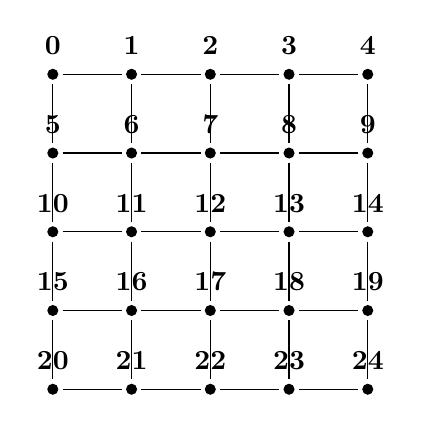
\begin{tikzpicture}
		\node[label=above:$\bf{0}$] (v0) at (0,0) {};\fill (v0) circle (2pt);
		\node[label=above:$\bf{1}$] (v1) at (1,0) {};\fill (v1) circle (2pt);
		\node[label=above:$\bf{2}$] (v2) at (2,0) {};\fill (v2) circle (2pt);
		\node[label=above:$\bf{3}$] (v3) at (3,0) {};\fill (v3) circle (2pt);
		\node[label=above:$\bf{4}$] (v4) at (4,0) {};\fill (v4) circle (2pt);
		
		\node[label=above:$\bf{5}$] (v5) at (0,-1) {};\fill (v5) circle (2pt);
		\node[label=above:$\bf{6}$] (v6) at (1,-1) {};\fill (v6) circle (2pt);
		\node[label=above:$\bf{7}$] (v7) at (2,-1) {};\fill (v7) circle (2pt);
		\node[label=above:$\bf{8}$] (v8) at (3,-1) {};\fill (v8) circle (2pt);
		\node[label=above:$\bf{9}$] (v9) at (4,-1) {};\fill (v9) circle (2pt);
	
		\node[label=above:$\bf{10}$] (v10) at (0,-2) {};\fill (v10) circle (2pt);
		\node[label=above:$\bf{11}$] (v11) at (1,-2) {};\fill (v11) circle (2pt);
		\node[label=above:$\bf{12}$] (v12) at (2,-2) {};\fill (v12) circle (2pt);
		\node[label=above:$\bf{13}$] (v13) at (3,-2) {};\fill (v13) circle (2pt);
		\node[label=above:$\bf{14}$] (v14) at (4,-2) {};\fill (v14) circle (2pt);
	
		\node[label=above:$\bf{15}$] (v15) at (0,-3) {};\fill (v15) circle (2pt);
		\node[label=above:$\bf{16}$] (v16) at (1,-3) {};\fill (v16) circle (2pt);
		\node[label=above:$\bf{17}$] (v17) at (2,-3) {};\fill (v17) circle (2pt);
		\node[label=above:$\bf{18}$] (v18) at (3,-3) {};\fill (v18) circle (2pt);
		\node[label=above:$\bf{19}$] (v19) at (4,-3) {};\fill (v19) circle (2pt);
	
		\node[label=above:$\bf{20}$] (v20) at (0,-4) {};\fill (v20) circle (2pt);
		\node[label=above:$\bf{21}$] (v21) at (1,-4) {};\fill (v21) circle (2pt);
		\node[label=above:$\bf{22}$] (v22) at (2,-4) {};\fill (v22) circle (2pt);
		\node[label=above:$\bf{23}$] (v23) at (3,-4) {};\fill (v23) circle (2pt);
		\node[label=above:$\bf{24}$] (v24) at (4,-4) {};\fill (v24) circle (2pt);
		
		\draw[-] (v0) to (v1); \draw[-]  (v0) to (v5);
		\draw[-] (v1) to (v2); \draw[-]  (v1) to (v6);
		\draw[-] (v2) to (v3); \draw[-]  (v2) to (v7);
		\draw[-] (v3) to (v4); \draw[-]  (v3) to (v8);
		\draw[-] (v4) to (v9);
		\draw[-] (v5) to (v6); \draw[-]  (v5) to (v10);
		\draw[-] (v6) to (v7); \draw[-]  (v6) to (v11);
		\draw[-] (v7) to (v8); \draw[-]  (v7) to (v12);
		\draw[-] (v8) to (v9); \draw[-]  (v8) to (v13);
		\draw[-] (v9) to (v14);
		\draw[-] (v10) to (v11); \draw[-]  (v10) to (v15);
		\draw[-] (v11) to (v12); \draw[-]  (v11) to (v16);
		\draw[-] (v12) to (v13); \draw[-]  (v12) to (v17);
		\draw[-] (v13) to (v14); \draw[-]  (v13) to (v18);
		\draw[-] (v14) to (v19);
	
		\draw[-] (v15) to (v16); \draw[-]  (v15) to (v20);
		\draw[-] (v16) to (v17); \draw[-]  (v16) to (v21);
		\draw[-] (v17) to (v18); \draw[-]  (v17) to (v22);
		\draw[-] (v18) to (v19); \draw[-]  (v18) to (v23);
		\draw[-] (v19) to (v24);
		\draw[-] (v20) to (v21);
		\draw[-] (v21) to (v22);
		\draw[-] (v22) to (v23);
		\draw[-] (v23) to (v24);
    \end{tikzpicture}}
\end{minipage}
\hfill
\begin{minipage}[h]{0.33\linewidth}
	\centering
    \vbox{ 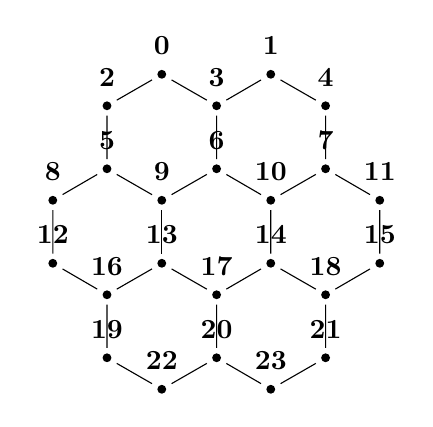
\begin{tikzpicture}[scale=0.8]
		\node[label=above:$\bf{0}$] (v0) at (0,0) {};\fill (v0) circle (2pt);
		\node[label=above:$\bf{1}$] (v1) at (1.73,0) {};\fill (v1) circle (2pt);

		\node[label=above:$\bf{2}$] (v2) at (-0.87,-0.5) {};\fill (v2) circle (2pt);
		\node[label=above:$\bf{3}$] (v3) at (0.87,-0.5) {};\fill (v3) circle (2pt);
		\node[label=above:$\bf{4}$] (v4) at (2.6,-0.5) {};\fill (v4) circle (2pt);
		
		\node[label=above:$\bf{5}$] (v5) at (-0.87,-1.5) {};\fill (v5) circle (2pt);
		\node[label=above:$\bf{6}$] (v6) at (0.87,-1.5) {};\fill (v6) circle (2pt);
		\node[label=above:$\bf{7}$] (v7) at (2.6,-1.5) {};\fill (v7) circle (2pt);

		\node[label=above:$\bf{8}$] (v8) at (-1.73,-2) {};\fill (v8) circle (2pt);
		\node[label=above:$\bf{9}$] (v9) at (0,-2) {};\fill (v9) circle (2pt);
		\node[label=above:$\bf{10}$] (v10) at (1.73,-2) {};\fill (v10) circle (2pt);
		\node[label=above:$\bf{11}$] (v11) at (3.46,-2) {};\fill (v11) circle (2pt);

		\node[label=above:$\bf{12}$] (v12) at (-1.73,-3) {};\fill (v12) circle (2pt);
		\node[label=above:$\bf{13}$] (v13) at (0,-3) {};\fill (v13) circle (2pt);
		\node[label=above:$\bf{14}$] (v14) at (1.73,-3) {};\fill (v14) circle (2pt);
		\node[label=above:$\bf{15}$] (v15) at (3.46,-3) {};\fill (v15) circle (2pt);

		\node[label=above:$\bf{16}$] (v16) at (-0.87,-3.5) {};\fill (v16) circle (2pt);
		\node[label=above:$\bf{17}$] (v17) at (0.87,-3.5) {};\fill (v17) circle (2pt);
		\node[label=above:$\bf{18}$] (v18) at (2.6,-3.5) {};\fill (v18) circle (2pt);

		\node[label=above:$\bf{19}$] (v19) at (-0.87,-4.5) {};\fill (v19) circle (2pt);
		\node[label=above:$\bf{20}$] (v20) at (0.87,-4.5) {};\fill (v20) circle (2pt);
		\node[label=above:$\bf{21}$] (v21) at (2.6,-4.5) {};\fill (v21) circle (2pt);

		\node[label=above:$\bf{22}$] (v22) at (0,-5) {};\fill (v22) circle (2pt);
		\node[label=above:$\bf{23}$] (v23) at (1.73,-5) {};\fill (v23) circle (2pt);

		
		\draw[-] (v0) to (v2); \draw[-]  (v0) to (v3);
		\draw[-] (v1) to (v3); \draw[-]  (v1) to (v4);
		\draw[-] (v2) to (v5); 
		\draw[-] (v3) to (v6);
		\draw[-] (v4) to (v7);
		\draw[-] (v5) to (v8); \draw[-] (v5) to (v9);
		\draw[-] (v6) to (v9); \draw[-] (v6) to (v10);
		\draw[-] (v7) to (v10);\draw[-] (v7) to (v11);
		\draw[-] (v8) to (v12);
		\draw[-] (v9) to (v13);
		\draw[-] (v10) to (v14);
		\draw[-] (v11) to (v15);
		\draw[-] (v12) to (v16);
		\draw[-] (v13) to (v16); \draw[-] (v13) to (v17);
		\draw[-] (v14) to (v17); \draw[-] (v14) to (v18);
		\draw[-] (v15) to (v18);
		\draw[-] (v16) to (v19);
		\draw[-] (v17) to (v20);
		\draw[-] (v18) to (v21);
		\draw[-] (v19) to (v22);
		\draw[-] (v20) to (v22); \draw[-] (v20) to (v23);
		\draw[-] (v21) to (v23);
    \end{tikzpicture}}
\end{minipage}
\hfill
\begin{minipage}[h]{0.33\linewidth}
	\centering
    \vbox{ 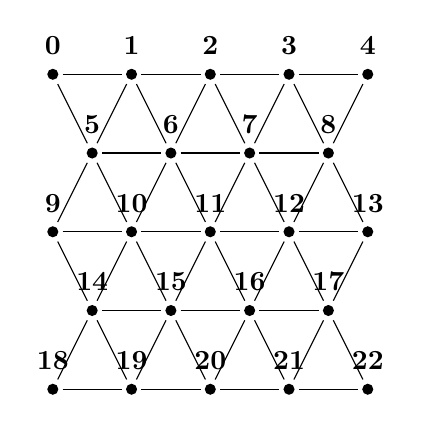
\begin{tikzpicture}
		\node[label=above:$\bf{0}$] (v0) at (0,0) {};\fill (v0) circle (2pt);
		\node[label=above:$\bf{1}$] (v1) at (1,0) {};\fill (v1) circle (2pt);
		\node[label=above:$\bf{2}$] (v2) at (2,0) {};\fill (v2) circle (2pt);
		\node[label=above:$\bf{3}$] (v3) at (3,0) {};\fill (v3) circle (2pt);
		\node[label=above:$\bf{4}$] (v4) at (4,0) {};\fill (v4) circle (2pt);
		
		\node[label=above:$\bf{5}$] (v5) at (0.5,-1) {};\fill (v5) circle (2pt);
		\node[label=above:$\bf{6}$] (v6) at (1.5,-1) {};\fill (v6) circle (2pt);
		\node[label=above:$\bf{7}$] (v7) at (2.5,-1) {};\fill (v7) circle (2pt);
		\node[label=above:$\bf{8}$] (v8) at (3.5,-1) {};\fill (v8) circle (2pt);
	
		\node[label=above:$\bf{9}$] (v9) at (0,-2) {};\fill (v9) circle (2pt);
		\node[label=above:$\bf{10}$] (v10) at (1,-2) {};\fill (v10) circle (2pt);
		\node[label=above:$\bf{11}$] (v11) at (2,-2) {};\fill (v11) circle (2pt);
		\node[label=above:$\bf{12}$] (v12) at (3,-2) {};\fill (v12) circle (2pt);
		\node[label=above:$\bf{13}$] (v13) at (4,-2) {};\fill (v13) circle (2pt);
	
		\node[label=above:$\bf{14}$] (v14) at (0.5,-3) {};\fill (v14) circle (2pt);
		\node[label=above:$\bf{15}$] (v15) at (1.5,-3) {};\fill (v15) circle (2pt);
		\node[label=above:$\bf{16}$] (v16) at (2.5,-3) {};\fill (v16) circle (2pt);
		\node[label=above:$\bf{17}$] (v17) at (3.5,-3) {};\fill (v17) circle (2pt);

	
		\node[label=above:$\bf{18}$] (v18) at (0,-4) {};\fill (v18) circle (2pt);
		\node[label=above:$\bf{19}$] (v19) at (1,-4) {};\fill (v19) circle (2pt);
		\node[label=above:$\bf{20}$] (v20) at (2,-4) {};\fill (v20) circle (2pt);
		\node[label=above:$\bf{21}$] (v21) at (3,-4) {};\fill (v21) circle (2pt);
		\node[label=above:$\bf{22}$] (v22) at (4,-4) {};\fill (v22) circle (2pt);
		
		\draw[-] (v0) to (v1); \draw[-]  (v0) to (v5);
		\draw[-] (v1) to (v2); \draw[-]  (v1) to (v5); \draw[-]  (v1) to (v6);
		\draw[-] (v2) to (v3); \draw[-]  (v2) to (v6); \draw[-]  (v2) to (v7);
		\draw[-] (v3) to (v4); \draw[-]  (v3) to (v7); \draw[-]  (v3) to (v8);
		\draw[-] (v4) to (v8);
		\draw[-] (v5) to (v6); \draw[-]  (v5) to (v9); \draw[-]  (v5) to (v10);
		\draw[-] (v6) to (v7); \draw[-]  (v6) to (v10); \draw[-]  (v6) to (v11);
		\draw[-] (v7) to (v8); \draw[-]  (v7) to (v11); \draw[-]  (v7) to (v12);
		\draw[-] (v8) to (v12); \draw[-]  (v8) to (v13);
		\draw[-] (v9) to (v10); \draw[-] (v9) to (v14);
		\draw[-] (v10) to (v11); \draw[-]  (v10) to (v14);\draw[-]  (v10) to (v15);
		\draw[-] (v11) to (v12); \draw[-]  (v11) to (v15);\draw[-]  (v11) to (v16);
		\draw[-] (v12) to (v13); \draw[-]  (v12) to (v16);\draw[-]  (v12) to (v17);
		\draw[-]  (v13) to (v17);
		\draw[-] (v14) to (v15); \draw[-] (v14) to (v18); \draw[-] (v14) to (v19);
		\draw[-] (v15) to (v16); \draw[-] (v15) to (v19); \draw[-] (v15) to (v20);
		\draw[-] (v16) to (v17); \draw[-] (v16) to (v20); \draw[-] (v16) to (v21);
		\draw[-] (v17) to (v21); \draw[-] (v17) to (v22);
		\draw[-] (v18) to (v19);
		\draw[-] (v19) to (v20);
		\draw[-] (v20) to (v21);
		\draw[-] (v21) to (v22);
    \end{tikzpicture}}
\end{minipage}
\begin{minipage}[ht]{1\linewidth}
\begin{tabular}{p{0.32\linewidth}p{0.32\linewidth}p{0.32\linewidth}}
\centering a) Square Lattice & \centering b) Hexagonal Lattice  & \centering c) Triangular Lattice \\
\end{tabular}
\end{minipage}
\caption{ Examples of lattice graphs}
\label{fig:2}
\end{figure} 

Maybe the hexagonal covering is the most common one. In this case the transmitters are assumed to be at the centers of the hexagons 
and two transmitters are adjacent in the graph 
if and only if the corresponding hexagons share a common 
edge. The graph constructed this way is a triangular lattice. 
Some research has been done for the classical frequency assignment problem on these graphs, see ~\cite{hex1,hex2,hex3,hex4,hex5}.


In our experiments we performed computations with the Euclidean model and with 
the graph model for three problem types arising from lattice graphs.  For the graph version the classical graph distance was taken, 
(e.g., the distance between~0 and~21 in the triangular lattice is~5). 
For the Euclidean version coordinates were given to the vertices such 
that every edge shown in~Fig.~\ref{fig:2} has length~1. 
So the coordinates for the vertices~$0$, $1$ and $2$ are 
$(-\frac{\sqrt{3}}{2},+\frac{3}{2})$, $(+\frac{\sqrt{3}}{2},+\frac{3}{2})$, 
$(-\sqrt{3},+1)$ in the hexagonal lattice, 
$(-2,+2)$, ($-1,+2)$, $(0,+2)$ in the square lattice and 
$(-2,+2)$, $(-1,+2)$, $(0,+2)$ in the triangular lattice. 
E.g., the distance between~0 and~1 in the hexagonal lattice is~$\sqrt{3}$. 

\begin{comment} 
\subsection*{Hexagonal lattice: } 
0($-\frac{\sqrt{3}}{2},+\frac{3}{2}$), 1($+\frac{\sqrt{3}}{2},+\frac{3}{2}$), 
2($-\sqrt{3},+1$), 3($0,1$), 4($+\sqrt{3},+1$), 5($-\sqrt{3},0$), 
6($0,0$), 7($+\sqrt{3},0$), 8($-\frac{3\cdot\sqrt{3}}{2},-\frac{1}{2}$), 
9($-\frac{\sqrt{3}}{2},-\frac{1}{2}$), 10($+\frac{\sqrt{3}}{2},-\frac{1}{2}$), 
11($+\frac{3\cdot\sqrt{3}}{2},-\frac{1}{2}$), 12($-\frac{3\cdot\sqrt{3}}{2},-\frac{3}{2}$), 
13($-\frac{\sqrt{3}}{2},-\frac{3}{2}$), 14($+\frac{\sqrt{3}}{2},-\frac{3}{2}$), 
15($+\frac{3\cdot\sqrt{3}}{2},-\frac{3}{2}$), 16($-\sqrt{3},-2$), 
17($0,-2$), 18($+\sqrt{3},-2$), 19($-\sqrt{3},-3$), 20($0,-3$), 
21($+\sqrt{3},-3$), 22($-\frac{\sqrt{3}}{2},-\frac{7}{2}$), 23($+\frac{\sqrt{3}}{2},-\frac{7}{2}$) 
\subsection*{Square lattice:} 
0($-2,+2$), 1($-1,+2$), 2($0,+2$), 3($+1,+2$), 4($+2,+2$), 5($-2,+1$), 
6($-1,+1$), 7($0,+1$), 8($+1,+1$), 9($+2,+1$), 10($-2,0$), 11($-1,0$), 
12($0,0$), 13($+1,0$), 14($+2,0$), 15($-2,-1$), 16($-1,-1$), 
17($0,-1$), 18($+1,-1$), 19($+2,-1$), 20($-2,-2$), 21($-1,-2$), 
22($0,-2$), 23($+1,-2$), 24($+2,-2$) 
\subsection*{Triangular lattice:} 
c, 3($+3,0$), 4($+4,0$), 5($+\frac{1}{2},+\frac{\sqrt{3}}{2}$), 
6($+\frac{3}{2},+\frac{\sqrt{3}}{2}$), 7($+\frac{5}{2},+\frac{\sqrt{3}}{2}$), 
8($+\frac{7}{2},+\frac{\sqrt{3}}{2}$), 9($0,+\sqrt{3}$), 10($+1,+\sqrt{3}$), 
11($+2,+\sqrt{3}$), 12($+3,+\sqrt{3}$), 13($+4,+\sqrt{3}$), 14($+\frac{1}{2},+\frac{3\cdot\sqrt{3}}{2}$), 
15($+\frac{3}{2},+\frac{3\cdot\sqrt{3}}{2}$), 16($+\frac{5}{2},+\frac{3\cdot\sqrt{3}}{2}$), 
17($+\frac{7}{2},+\frac{3\cdot\sqrt{3}}{2}$), 18($0,+2\cdot\sqrt{3}$), 
19($+1,+2\cdot\sqrt{3}$), 20($+2,+2\cdot\sqrt{3}$), 21($+3,+2\cdot\sqrt{3}$), 
22($+4,+2\cdot\sqrt{3}$) 
\end{comment} 


The difference of the distance between two vertices in the Euclidean and in the 
graph model can be small or zero, but also relatively high. 
Two vertices with graph distance~4 could, for example, have Euclidean distance 4, 
$\sqrt{10}$ or $\sqrt{8}$. 

With the help of the transformation function~$\ell$ we tried to have a similar 
range of spans for the graph and the corresponding Euclidean model. 
Of course, $\ell$ has to be monotonically decreasing. We experimented with 
two variants for~$\ell$ which in addition have the property that the values for 
integer distances are preserved. i.e.\ $\ell(\dist(u,v))=j_{\dist(u,v)}$ for $\dist(u,v)$ integer. 
E.g., this is satisfied by defining $\ell(\dist(u,v))=j+1-\dist(u,v)$ for 
$L(j,j-1,\ldots ,1)-$labelings. 
Since the graph distances are not smaller than the Euclidean distances, the 
spans for the graph problems will be higher in general. 

\section{First computational experiments} 

For our computations we consider the square lattice on 25~vertices, the hexagonal 
lattice on 24~vertices and the triangular lattice on 23~vertices (as depicted in Fig.~\ref{fig:2}). 
The minimum spans have been computed with ILOG CPLEX Version 12.4.1~\cite{Cpl15}. 

All computations were done on a computer with $4$ processors Intel Core $i7-2600$, $3.40$ GHz, and $16$GB RAM. The implementation is in C++. 

\subsection{Classical model} 

In a first step we wanted to determine problem sizes which can be solved in reasonable time with the classical model (\ref{ip:1}) - (\ref{ip:4}). 
For this, we tested the model on the three types of lattices with different numbers of nodes. The running times (in min:sec) and the respective optimal solutions are presented in Table \ref{tab:00}. 

One can see, that already for the triangular lattice with $30$ nodes computation of an optimal $L(3,2,1)-$labeling takes hours. The computation of an optimal $L(4,3,2,1)-$labeling exhausted all computer resources and was aborted. 

\begin{table}[h] 
\centering 

\begin{tabular}{|r||r|r||r|r||r|r|} 
\hline 
Lattice  & \multicolumn{2}{c||}{$L(2,1)$} & \multicolumn{2}{c||}{$L(3,2,1)$} & \multicolumn{2}{c|}{$L(4,3,2,1)$} \\ 
         & Span & CPU & Span & CPU & Span & CPU  \\ 
\hline 
Hexagonal ($24$ nodes)  & 5 & 0.2 & 9 & 1.0 & 19 & 47.1  \\ 
\hline 
Hexagonal ($30$ nodes)  & 5 & 0.3 & 9 & 1.9 & 20 & 8:11.4  \\ 
\hline 
Triangular ($23$ nodes) & 8 & 0.9 & 18 & 9:33.5 & 32 & 15575:50  \\ 
\hline 
Triangular ($30$ nodes) & 8 & 1.7 & 18 & 163:50.7 & - & -      \\ 
\hline 
Square ($25$ nodes)    & 6 & 0.6 & 11 & 1.72 & 25 & 143:39.05  \\ 
\hline 
Square ($30$ nodes)    & 6 & 1.1 & 11 & 2.3 & 25 & 335:24.8      \\ 
\hline 
\end{tabular} 
\caption{ Spans and running time using the classical model (\ref{ip:1})-(\ref{ip:4})} 
\label{tab:00} 
\end{table} 

We also tested if different values of $j_1$, $j_2$ in the $L(j_1,j_2)-$labeling have an influence on the running time. The computation of $L(3,2)-$labelings took longer than the computation of $L(2,1)-$labeling for almost all considered graphs (see Table~\ref{tab:01}). 
 

\begin{table}[h] 
\centering 
\begin{tabular}{|r||r|r||r|r|} 
\hline 
Lattice  & \multicolumn{2}{c||}{$L(2,1)$} & \multicolumn{2}{c|}{$L(3,2)$}\\ 
         & Span & CPU & Span & CPU\\ 
\hline 
Hexagonal ($24$ nodes)  & 5 & 0.2 & 9 & 0.42 \\ 
\hline 
Hexagonal ($30$ nodes)  & 5 & 0.3 & 9 & 1.04 \\ 
\hline 
Triangular ($23$ nodes) & 8 & 0.9 & 16 & 18.00 \\ 
\hline 
Triangular ($30$ nodes) & 8 & 2.6 & 16 & 19.23 \\ 
\hline 
Square ($25$ nodes)    & 6 & 0.6 & 11 & 2.24 \\ 
\hline 
Square ($30$ nodes)  & 6 & 1.1 & 11 & 1.30 \\ 
\hline 
\end{tabular} 
\caption{$L(3,2)$ vs $L(2,1)$} 
\label{tab:01} 
\end{table} 

\subsection{Linear transformation} 

We first considered $L(2,1)$- and $L(3,2,1)$-labelings for the classical model (\ref{ip:1})-(\ref{ip:4}) and used functions $\ell_{2}(\dist(u,v))=3-\dist(u,v)$ and $\ell_{3}(\dist(u,v))=4-\dist(u,v)$ 
in the respective Euclidean model. 
The distance of adjacent vertices is~1 in both cases, 
the distance beween non-adjacent vertices can be the same as their graph distance, 
but also considerably smaller. Because of this, the constraints for most vertex 
pairs are stronger in the Euclidean model. 

\noindent 
Table~\ref{tab:2} gives the spans and running times as obtained with Cplex. 
The spans between the models differ as expected. 
Surprisingly, the running times for the Euclidean model are considerably higher. 

\begin{table}[h] 
\begin{center} 
\renewcommand{\arraystretch}{1.3} 
\renewcommand{\tabcolsep}{8pt} 
\begin{tabular}{|r||r|r|r|r||r|r|r|r|} 
\hline 
Lattice  & \multicolumn{2}{c|}{$L(2,1)$} & \multicolumn{2}{c||}{Euclidean} & 
 \multicolumn{2}{c|}{$L(3,2,1)$} & \multicolumn{2}{c|}{Euclidean}\\ 
  & Span & CPU & Span & CPU & Span & CPU & Span & CPU\\ 
\hline 
Hexagonal   & 5 & 0.2 & 6.42 & 4.6 & 9 & 0.9& 16.62 & 92:57.7 \\ 
\hline 
Triangular  & 8 & 0.9 & 9.78 & 38.6 & 18 & 9:33.5& 21.91 & 6149:18.0 \\ 
\hline 
Square     & 6 & 0.6 & 8.64  & 15.3 & 11 & 1.7 & 19.91 & 2559:47.0  \\ 
\hline 
\end{tabular} 
\end{center} 
\caption{Spans and running times for the linear function} 
\label{tab:1} 
\end{table} 

\subsection{Stepwise transformation} 

With this type of function we want to map the Euclidean distances to integer 
values, again preserving the value if the distance is integer already. 

Table~\ref{tab:2} shows the possible Euclidean distances for the three lattices 
and the corresponding graph distances. 

\begin{table}[h] 
\begin{center} 
\renewcommand{\arraystretch}{1.3} 
\renewcommand{\tabcolsep}{8pt} 
\begin{tabular}{|r|r||r|r||r|r|} 
\hline 
\multicolumn{2}{|c||}{Hexagonal} & \multicolumn{2}{c||}{Triangular} & \multicolumn{2}{c|}{Square} \\ 
 Euclidean & Graph & Euclidean & Graph & Euclidean & Graph\\ 
\hline 
$1$                              & 1  & $1$                              & 1 & $1$ & 1\\ 
$\sqrt{3}$                    & 2   & $2,\sqrt{3}$                 & 2 & $2,\sqrt{2}$ & 2\\ 
$2,\sqrt{7}$                 & 3   & $3,\sqrt{7}$                 & 3 & $3,\sqrt{5}$ & 3\\ 
$3,2\sqrt{3}$               & 4   & $4,\sqrt{13},2\sqrt{3}$ & 4 & $4,\sqrt{10},2\sqrt{2}$ & 4\\ 
$4,\sqrt{13},\sqrt{19}$ & 5  & $\sqrt{19},\sqrt{21}$    & 5 & $\sqrt{13},\sqrt{17}$ & 5\\ 
$\sqrt{21},3\sqrt{3}$   & 6   & $2\sqrt{7}$                  & 6 & $2\sqrt{5},3\sqrt{2}$ & 6\\ 
$5,2\sqrt{7}$               & 7  &                                     &   & $5$ & 7\\ 
                               &     &                                         &   & $4\sqrt{2}$ & 8\\ 
\hline 
\end{tabular} 
\end{center} 
\caption{Euclidean and graph distances for the three lattices}\label{tab:2} 
\end{table} 

For the hexagonal lattice here are some vertex pairs with Euclidean distance $3\sqrt{3}$ 
and graph distance 6, and some with Euclidean distance 5 and graph 
distance 7. For these pairs the graph distance is longer although the 
Euclidean is shorter. For the square lattice there are for example 
pairs with Euclidean distance $2\sqrt{2}$ 
and graph distance 4, and some with Euclidean distance 3 and graph 
distance 3. For the triangular lattice there are no such exceptions. 

Let $f(x)$ denote the graph distance corresponding to the Euclidean distance (in the 
respective lattice). 
For $L(2,1)$- and $L(3,2,1)$-labelings only the graph distances 1, 2 and 3 have to be taken into account. 
For the respective pairs we set $\ell_2(\dist(u,v))=3-f(\dist(u,v)))$ 
for $L(2,1)$-labelings and $\ell_3(\dist(u,v))=4-f(\dist(u,v)))$ for $L(3,2,1)$-labelings. 

Table~\ref{tab:3} shows spans and running times for these step functions. 
Although the constraints are the same for each vertex pair in this case, the calculations 
are still much slower in the Euclidean model. However, compared with the 
previous section (see Table~\ref{tab:1}) they have improved a lot. 

\begin{table}[h] 
\begin{center} 
\renewcommand{\arraystretch}{1.3} 
\renewcommand{\tabcolsep}{8pt} 
\begin{tabular}{|r||r|r|r|r||r|r|r|r|} 
\hline 
Lattice  & \multicolumn{2}{c|}{$L(2,1)$} & \multicolumn{2}{c||}{Euclidean} & 
 \multicolumn{2}{c|}{$L(3,2,1)$} & \multicolumn{2}{c|}{Euclidean}\\ 
  & Span & CPU & Span & CPU & Span & CPU & Span & CPU\\ 
\hline 
Hexagonal & 5 & 0.2 & 5 & 2.2 & 9 & 0.9 & 9 & 3.8 \\ 
\hline 
Triangular  & 8 & 0.9 & 8 & 27.3 & 18 & 9:33.5 & 18 & 76:39.1 \\ 
\hline 
Square     & 6 & 0. & 6  & 23.0 & 11 & 1.7 & 11 & 10.2  \\ 
\hline 
\end{tabular} 
\end{center} 
\caption{Spans and running times for the step function}\label{tab:3} 
\end{table} 

\section{Model improvements} 

As one can see from the previous section, computing an optimal $L(2,1)-$ and an $L(3,2,1)-$labeling for the considered lattice graphs takes a lot of time. One 
of the reasons for this unsatisfactory performance is the bad quality of lower bounds in the optimization process (see Fig.\ref{fig:3}). In this section we discuss our attempts to improve the performance. 

All computations have been performed for the linear transformation function. 

% Fig 3 
\begin{figure}[h]
    \subfigure[$L(2,1)$ Labeling, optimal value $8.78029$]{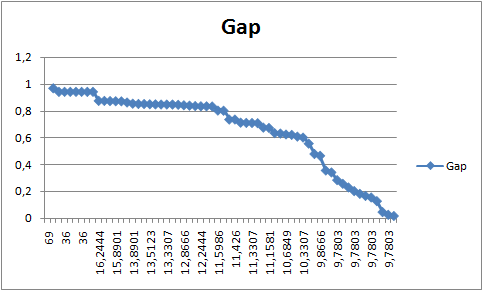
\includegraphics[width=0.49\textwidth]{figures/Triang_Lattice_L21_gap.png}}
    \subfigure[$L(3,2,1)$ Labeling, optimal value $21.9068$]{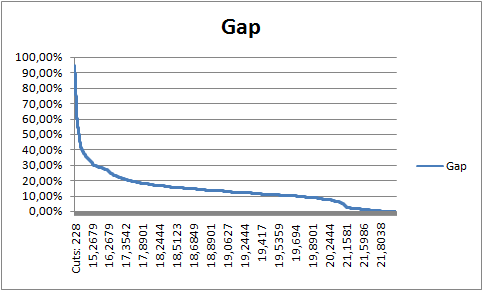
\includegraphics[width=0.49\textwidth]{figures/Triang_Lattice_L321_gap.png}}
\caption{Evolution of the LB in case of triangular lattice graph and real number labeling}
\label{fig:3}
\end{figure} 
 

\FloatBarrier 

\subsection{Reducing the value of $M$} 

It is well-known that whenever a linear model contains a so-called \emph{big M} 
it is usually advantageous to find the smallest possible value for~$M$. 
A speed-up of the computations can be expected. However, this is not 
guaranteed and the effect can also be reverse. 

\begin{comment} 
A good value for $M$ is clearly not smaller than the value that CPLEX 
would find for $\lambda+j_1$. But with this property it should 
be as small as possible since the bigger the value of $M$ is, the 
larger the size of the search space. The fact is that we have more 
inequalities, in this point the problem should be more complex. But 
the other side, these inequalities can help in the process of Branch-and-Bound, 
that can make the calculations faster. So, it should be tried to see 
whether the modification is effective in some cases. For this purpose, 
we must be able to estimate the results. A correct estimation of the 
value multiplied by a constant is already useful (if it is smaller 
than the original $M$-value). 
\end{comment} 

Since the optimum values from the classical 
model are available, it is easy to get good $M$ values for the Euclidean 
model. In the case $\ell_{2}(dist)=3-dist$ we set $M_{2}^{*}=2\cdot\lambda_{L(2,1)}$, 
while $M_{3}^{*}=3\cdot\lambda_{L(3,2,1)}$ in the case $\ell_{3}(dist)=4-dist$. 

Table~\ref{tab:4} compares  running times with those of Table~\ref{tab:1}. 
The new CPU times as well as the percentage of these times compared to 
those of Table~\ref{tab:1} are given. 

\begin{table}[h] 
\begin{center} 
\renewcommand{\arraystretch}{1.3} 
\renewcommand{\tabcolsep}{10pt} 
\begin{tabular}{|r||r|r||r|r|} 
\hline 
Lattice  & \multicolumn{2}{c||}{$L(2,1)$} & \multicolumn{2}{c|}{$L(3,2,1)$} \\ 
  & CPU & \% & CPU & \%\\ 
\hline 
Hexagonal & 5.2 & 113.0 & 104:43.5 & 112.7 \\ 
\hline 
Triangular  & 30.3 & \textbf{78.5} & 3519:4.4 & \textbf{57.2} \\ 
\hline 
Square      & 23.7 & 155.0 & 1416:30.2 & \textbf{55.3} \\ 
\hline 
\end{tabular} 
\end{center} 
\caption{Effect of new setting of $M$}\label{tab:4} 
\end{table} 

One can see that the modification works fairly well for the triangular 
lattice, but rather poorly for the hexagonal lattice. For the square lattice 
we have mixed results. 

\begin{comment} 
\subsection{Upper and lower bounds for the optimum} 

Another approach is to include some good upper and lower bounds for 
$\lambda$ in the formulation. In our case, of course, the proper 
upper bound is in question. We used the algorithm of binary search 
for determining it. The idea is to contract the lower and the upper 
bound as long as the gap between them (upper bound minus lower bound) 
is small enough. And the optimization may start only after this process 
with the received limits. We took the value received from CPLEX in 
the classical model for the initial lower bound, while we multiplied 
it by 2 in the case of $\ell_{2}(dist)$, and by 3 in the case of 
$\ell_{3}(dist)$, for the initial upper bound. In each iteration 
either the lower bound is attempted to move upward or the upper bound 
down. There is an admissibility problem solved each time. We set the 
required gap to 0.5. Our results are shown in the following table 
(only the running times are indicated, since the outcomes are the 
same in both cases as above): 

\begin{center} 
\begin{tabular}{|c|c|c|} 
\hline 
Lattice & $\ell_{2}(dist)=3-dist$ , new (s) & $\ell_{2}(dist)=3-dist$ , old (s)\\ 
\hline 
\hline 
Hexagonal & 13.28+135.43=148.71  & 4.57 \\ 
\hline 
Triangular & 447.24+883.27=1330.51 & 38.62 \\ 
\hline 
Square & 118.89+198.25=317.14 & 15.34 \\ 
\hline 
\multicolumn{1}{c}{ 
} & \multicolumn{1}{c}{ 
} & 
\\ 
\hline 
Lattice & $\ell_{3}(dist)=4-dist$ , new (s) & $\ell_{3}(dist)=4-dist$ , old (s)\\ 
\hline 
\hline 
Hexagonal & 337947+410468=748414  & 5777.68 \\ 
\hline 
Triangular & --- & 103883 \\ 
\hline 
Square & --- & 27793.8 \\ 
\hline 
\end{tabular} 
\par\end{center} 

The first addend in the sum is the running time needed for the calculation 
of the bounds, while the second one is the running time needed for 
the optimization itself. Incontrary to the expectations, the method 
did not improve the program, and even slowed it. And in addition, 
after the reduction of the feasible set, it is difficult to cut off 
some branches in the search tree (Bounding). Therefore the optimum 
search takes longer time than previously. 
\end{comment} 

\subsection{Strengthening the model} 

The inequalities in the above models are straightforward and we are 
interested in strengthening them. Let $G^\prime$ be a node induced subgraph of $G$. 
If we consider feasible labelings for $G^\prime$ then any constraint on the 
labels for $G^\prime$ is valid for all subgraphs of $G$ isomorphic to $G^\prime$. 
In the following we have chosen the smallest possible sum of the labels 
for $G^\prime$ as constraint, i.e., if $s(G)$ is the smallest sum of 
feasible labels for $G^\prime$ then the inequality $\sum_{v\in V(H)}c(v)\geq s(G)$ 
is valid for all subgraphs $H$ of $G$ isomorphic to $G^\prime$. 
We have experimented with several types of subgraphs. 

A \emph{star} is a graph $G=(V,E)$ such that $E=\{vw\mid w\in V\setminus\{v\}\}$ for some $v\in V$ 
(center vertex of the star). Suppose $|V|=m$. 
The sum of labels for a star is a lower bound for the sum of labels of every subgraph 
containing a star. Consider an $L(j_1,j_2,\ldots)$-labeling. For the star $m$ labels have 
to be chosen such that the gap between the label 
of the central vertex and the label of any other vertex is at least 
$j_1$, and the gap between the labels of any two non-central vertices 
is at least $j_2$. We distinguish three cases. 
\begin{enumerate} 
\item 
The label of the center is the smallest one. 
\item[]Then the labels are 0, $j_1$, 
$j_1+j_2$, $j_1+2j_2$, $j_1+3j_2$,\ldots , $j_1+(m-2)j_2$ 
summing up to $(m-1)\cdot j_1+\sum_{i=1}^{m-2}i\cdot j_2$. 
\item 
The label of the center is the greatest one. 
\item[]Then the labels are 0, $j_2$, 
$2j_2$,\ldots , $(m-2)j_2$, $(m-2)j_2+j_1$ with sum 
$(\sum_{i=1}^{m-2}i\cdot j_2)+(m-2)j_2+j_1$. 
\item 
The central label is the $(k+1)$st greatest label for some $k\ge1$. 
\item[]In this case the labels 0, $j_2$, 
$2j_2$,\ldots , $(k-1)j_2$, $(k-1)j_2+j_1$, $(k-1)j_2+2j_1$, 
$k\cdot j_2+2j_1$,\ldots , $(m-3)j_2+2j_1$ and their sum is 
$(\sum_{i=1}^{m-3}i\cdot j_2)+2(k-1)j_2+(2(m-k-1)+1)\cdot j_1$. 
\end{enumerate} 
Since $j_1\geq j_2$, an easy calculation shows that the smallest sum is obtained 
in case~2 and is equal to $\frac{1}{2}(m+1)(m-2)\cdot j_2+j_1$. 
So for every vertex $u\in V$ we can add its associated \emph{star inequality} 
\[ 
c(u)+\sum_{i\in N(u)}c(i)\geq\frac{(\deg(u)+2)(\deg(u)-1)}{2}\cdot j_2+j_1 
\] 
to the models (where $N(u)$ denotes the set of neighbors of~$u$ 
and $\deg(u)$ is the degree of~$u$. 

A second possibility is to associate inequalities with small 
sublattices of the lattices we considered in our computational experiments. 
We considered the triangles 
with side length 1, 2 and 3, the hexagons with side length 1 and 2, trapezes 
as half of a hexagon, squares with side length 1, 2 and 3, 
and small square lattices with 4 and 9 vertices. Table~\ref{tab:5} gives the 
smallest sums of labels for these subgraphs for the labelings $L(2,1)$ and $L(3,2,1)$. 

\begin{table}[h] 
\begin{center} 
\renewcommand{\arraystretch}{1.3} 
\renewcommand{\tabcolsep}{8pt} 
\begin{tabular}{|r||r||r|} 
\hline 
Sublattice & L(2,1)  & L(3,2,1) \\ 
\hline 
Hexagon with side length 1 & 16.61 & 31.61\\ 
\hline 
Hexagon with side length 2 & 3.00 & 10.82\\ 
\hline 
Trapeze with side length 1 & 7.0718 & 13.07\\ 
\hline 
Triangle with side length 1 & 6.00 & 9.00\\ 
\hline 
Triangle with side length 2 & 3.00 & 6.00\\ 
\hline 
Triangle with side length 3 & 0.00 & 3.00\\ 
\hline 
Square 1$\times$1 (4 vertices) & 10.34 & 16.34\\ 
\hline 
Square 2$\times$2 (4 vertices) & 2.69 & 8.69\\ 
\hline 
Square 3$\times$3 (4 vertices) & 0.00 & 2.00\\ 
\hline 
Square lattice 2$\times$2 (9 vertices) & 29.19 & 59.40\\ 
\hline 
Square lattice 1$\times$2 (6 vertices) & 16.23 & 30.28\\ 
\hline 
\end{tabular} 
\end{center} 
\caption{Minimum label sums for sublattices}\label{tab:5} 
\end{table} 

We examined the effect of the addition of these small subgraph inequalities. 
The results are presented in Table~\ref{tab:6} for the hexagonal, in Table~\ref{tab:7} 
for the triangular, and in Table~\ref{tab:8} for the square lattice. 
For the square lattice we only added non-overlapping squares which is only a small 
subset of possible squares. 

\begin{table}[h] 
\begin{center} 
\renewcommand{\arraystretch}{1.3} 
\renewcommand{\tabcolsep}{8pt} 
\begin{tabular}{|r||r||r|} 
\hline 
Hexagonal lattice & L(2,1) & L(3,2,1) \\ 
\hline
Without any subgraph-inequality   & 4.6 & 92:57.7\\ 
\hline 
Hexagons with side length 1       & 4.3 & 265:52.0\\ 
\hline 
Hexagons with side length 1 and 2 & 4.4 & 148:0\\ 
\hline 
Trapezes                          & 6.8 & 118:24.6\\ 
\hline 
\end{tabular} 
\end{center} 
\caption{Effect of subgraph inequalities for the hexagonal lattice}\label{tab:6} 
\end{table} 

\begin{table}[h] 
\begin{center} 
\renewcommand{\arraystretch}{1.3} 
\renewcommand{\tabcolsep}{8pt} 
\begin{tabular}{|r||r||r|} 
\hline 
Triangular lattice & L(2,1) & L(3,2,1) \\ 
\hline 
Without any subgraph-inequality & 38.6 & 6149:18.0\\ 
\hline 
Triangles with side length 1 & 21.0 & 4914:18.8\\ 
\hline 
Triangles with side length 1,2 and 3 & 37.2 & 9059:15.6\\ 
\hline 
Hexagons with side length 1 & 36.6 & 2519:20.3 \\ 
\hline 
\end{tabular} 
\end{center} 
\caption{Effect of subgraph inequalities for the triangular lattice}\label{tab:7} 
\end{table} 

\begin{table}[h] 
\begin{center} 
\renewcommand{\arraystretch}{1.3} 
\renewcommand{\tabcolsep}{8pt} 
\begin{tabular}{|r||r||r|} 
\hline 
Square lattice & L(2,1) & L(3,2,1) \\ 
\hline 
Without any subgraph-inequality       & 15.3 & 2559:47\\ 
\hline 
Squares with side length 1            & 24.3 & 3046:6.4\\ 
\hline 
Squares with side length 1,2 and 3    & 24.6 & 4424:14.7\\ 
\hline 
Rectangle with side length 1$\times$2 & 33.2 & {\it killed}\\ 
\hline 
\end{tabular} 
\end{center} 
\caption{Effect of subgraph inequalities for the square lattice}\label{tab:8} 
\end{table} 

For the hexagonal lattice we observe a running time improvement of about 10-20\%. 
In the triangular case, time reduces to about 50\% in two cases for the $L(3,2,1)$-labeling. 
Also in one case for the square lattice a considerable improvement is achieved. 

\section{Conclusions} 

We tried some further heuristics like numbering the vertices randomly in order 
to see if this makes a difference to CPLEX. But no consistent improvement 
could be observed. 

\begin{thebibliography}{1} 
 

\bibitem{hex5}K. Aardal, S.P.M. van Hoesel, A.M.C.A. Koster, C. Mannino, A. Sassano. Models and solution techniques for frequency assignment problems. Quarterly Journal of the Belgian, French and Italian Operations Research Societies, 1 (4) (2003), 261-317

\bibitem{10}H.L. Bodlaender, T. Kloks, R.B. Tan, J. van Leeuwen. 
Approximations for $\lambda-$coloring of graphs. The Computer Journal 
47 (2004), 193-204  

\bibitem{hex2}R. Borndoerfer, A. Eisenblaetter, M. Groetschel, A. Martin. Frequency assignment in cellular phone networks. Annals of Operations Research 76 (1998), 73-93

\bibitem{3}T. Calamoneri. The $L(h,k)-$labelling problem: 
An updated survey and annotated bibliography. Comput. J. 54 (2011), 
1344-1371 (A later version is available online at http://wwwusers.di.uniroma1.it/\textasciitilde{}calamo/PDF-FILES/survey.pdf) 

\bibitem{8}G.J. Chang, W.T. Ke, D. Kuo, D.D.F. Liu, R.K. Yeh. 
On L(d,1)-labelings of graphs. Discrete Math., 220 (2000), 57-66 

\bibitem{9}G.J. Chang, D. Kuo. The L(2,1)-labeling on graphs. 
SIAM J. Discrete Math., 9 (1996), 309-316 

\bibitem{CEHZ}G. Chartrand, D. Erwin, F. Harary, P. Zhang. Radio labelings of graphs. Bull. Inst. Combin. Appl. 33 (2001), 77-85

\bibitem{6}M.L. Chia, D. Kuo, H.Y. Liao, C.H. Yang, R.K. Yeh. 
$L(3,2,1)-$labeling of graphs, Taiwanese J. Math. 15 (2011), 
2439-2457 

\bibitem{hex4}F.Y.L. Chin, Y. Zhang, H. Zhu. A 1-local 13/9-competitive algorithm for multicoloring hexagonal graphs. Proc. 13th Annual International Computing and Combinatorics Conf. COCOON) (2007), 526-536

\bibitem{Cpl15} 
CPLEX Optimizer, \texttt{www.cplex.com}

\bibitem{12}N. Eggemann, F. Havet, S.D. Noble. k-L(2,1)-labelling 
for planar graphs is NP-complete for k$\geq$4. Disc. Appl. Math., 
158 (16) (2010), 1777-1788  

\bibitem{7} J. Fiala, P.A. Golovach, J. Kratochv\'i­l. Computational 
complexity of the distance constrained labeling problem for trees. 
Proc. 35th ICALP , Part I (2008), 294-305 

\bibitem{11}J. Fiala, P.A. Golovach, J. Kratochv\'i­l. Distance 
constrained labelings of graphs of bounded treewidth. Proc. 32th ICALP (2005), 
360-372  

\bibitem{G}J. A. Gallian. A dynamic survey of graph labeling. Electronic Journal of Combinatorics, (2014) \#DS6, 308 pages. 

\bibitem{13}J. R. Griggs, X.T. Jin. Real number graph labellings with distance conditions. 
SIAM J. Discrete Math., 20 (2006), 302-327 

\bibitem{GY92} 
J.R. Griggs, R.K. Yeh. Labeling graphs with a condition 
at distance two. SIAM J. Discrete Math., 5 (1992), 586-595 

\bibitem{HT}V. Hal\'asz, Zs. Tuza. Distance-constrained labeling of complete trees. Discrete Mathematics 338 (2015), 1398-1406

\bibitem{Hal80} 
W.K. Hale. Frequency assignment: Theory and application. 
Proc. IEEE, 68 (1980), 1497-1504

\bibitem{LMZ}X. Li, V. Mak, S. Zhou. Optimal radio labellings of complete m-
 ary trees, Discrete Applied Math. 158 (2010), 507-515

\bibitem{L}D. D.F. Liu. Radio number for trees Discrete Math. 308 (2008), 1153-1164

\bibitem{hex3}L. Narayanan, S.M. Shende. Static frequency assignment in cellular networks. Algorithmica, 29 (3) (2001), 396-409

\bibitem{hex1}S. Rajasekaran, K. Naik, D. Wei. On frequency assignment in cellular networks. DIMACS Series in Discrete Mathematics and Theoretical Computer Science 52 (2000), 293-302

\bibitem{5}Z. Shao. The $L(d_{1},d_{2},d_{3})-$labeling on 
graphs, J. Nanjing Univ. Math. Biquart. 21 (2004), 234-238 

\bibitem{4}Z.D. Shao, J.Z. Liu. The $L(3,2,1)-$labeling 
problem on graphs. Math. Appl. 17 (2004), 596-602 



\end{thebibliography} 

\end{document} 
